\documentclass[conference]{IEEEtranch}
\ifCLASSINFOpdf
   \usepackage[pdftex]{graphicx}
   \DeclareGraphicsExtensions{.pdf,.jpeg,.png}
\else
\fi
% correct bad hyphenation here
\hyphenation{op-tical net-works semi-conduc-tor infra-structure high-lighted asses-sment inter-action as-sess-ment}
%\usepackage{array,ragged2e}

%\usepackage[T1]{fontenc}
%\usepackage[latin1]{inputenc}
\usepackage{ctex}
%\usepackage[english]{babel}

\usepackage{multirow}
\usepackage{tabularx,calc}
%\usepackage{amsmath}
\usepackage{color}
\usepackage{colortbl}


\renewcommand{\contentsname}{Contents}
\renewcommand{\figurename}{图}
\renewcommand{\abstractname}{摘要}
\usepackage{hyperref}

\usepackage{tikz,amsmath, amssymb,bm,color}
\usepackage{pgfplots}
\usepackage{environ}
\usepackage{ifthen}
\makeatletter
\newsavebox{\measure@tikzpicture}
\NewEnviron{scaletikzpicturetowidth}[1]{%
	\def\tikz@width{#1}%
	\def\tikzscale{1}\begin{lrbox}{\measure@tikzpicture}%
		\BODY
	\end{lrbox}%
	\pgfmathparse{#1/\wd\measure@tikzpicture}%
	\edef\tikzscale{\pgfmathresult}%
	\BODY
}
\makeatother
\newboolean{compileforpublish}
\setboolean{compileforpublish}{true}
\newboolean{isaccepted}
\setboolean{isaccepted}{true}
%copyrightnotice IEEE with tikz
\ifthenelse{\boolean{isaccepted}}
{%if
	\newcommand\copyrighttext{%
		\footnotesize \parbox[t]{.11\textwidth}{\copyright{} \the\year~IEEE.} \parbox[t]{.89\textwidth}{}}
}
{%else
	\newcommand\copyrighttext{%
		\footnotesize \centering This work has been submitted to the IEEE for possible publication.\\ Copyright may be transferred without notice, after which this version may no longer be accessible.}
}

\newcommand\copyrightnotice{%
	\ifthenelse{\boolean{compileforpublish}}
	{
		\begin{tikzpicture}[remember picture,overlay]
		\node[anchor=south,yshift=10.5pt] at (current page.south) {\parbox{\dimexpr\textwidth-\fboxsep-\fboxrule\relax}{\copyrighttext}};
		\end{tikzpicture}%
	}
}

\newcommand{\contradiction}{{\hbox{%
			\setbox0=\hbox{$\mkern-3mu\times\mkern-3mu$}%
			\setbox1=\hbox to0pt{\hss$\times$\hss}%
			\copy0\raisebox{0.5\wd0}{\copy1}\raisebox{-0.5\wd0}{\box1}\box0
}}}

\renewcommand{\IEEEtitletopspaceextra}{20pt}

\begin{document}
%
\title{用于自动驾驶汽车开发、测试与验证的场景}

\author{\IEEEauthorblockN{Till Menzel, Gerrit Bagschik and Markus Maurer}
\IEEEauthorblockA{Institute of Control Engineering\\
Technische Universit\"at Braunschweig\\
Braunschweig, Germany\\
}
}


\maketitle%
\copyrightnotice%

\begin{abstract}
	%Einleitender Satz?
%The latest version of the ISO~26262 standard from 2016 represents the state of the art for a safety-guided development of safety-critical electric/electronic vehicle systems.
%These vehicle systems include advanced driver assistance systems and vehicle guidance systems.
%The development process proposed in the ISO~26262 standard is based upon multiple V-models, and defines activities and work products for each process step.
%In many of these process steps, scenario based approaches can be applied to achieve the defined work products for the development of automated driving functions.
%To accomplish the work products of different process steps, scenarios have to focus on various aspects like a human understandable notation or a description via state variables.
%This leads to contradictory requirements regarding the level of detail and way of notation for the representation of scenarios.
%In this paper, the authors discuss requirements for the representation of scenarios in different process steps defined by the ISO~26262 standard, propose a consistent terminology based on prior publications for the identified levels of abstraction, and demonstrate how scenarios can be systematically evolved along the phases of the development process outlined in the ISO~26262 standard.

2016年更新的ISO~26262标准,代表了车辆安全的关键电气/电子系统安全指导开发的最新技术,可以应用于高级驾驶辅助系统(ADAS)和自动驾驶系统的开发和验证。标准规定了基于V型开发模式的各个阶段所要求的工作内容和输出产品。在V型开发模式的各个阶段,均可应用基于场景的方法,来获得相应的工作输出产品。为了完成各个阶段的工作产品,场景必须关注各种方面,如人类可理解的符号或通过状态变量的描述。
在应用基于场景的方法时,不同开发阶段对场景细节程度和场景描述方式的需求存在矛盾。本文作者讨论了ISO 26262标准中不同阶段对场景描述的要求,提出了满足一致性的场景描述方法,并演示了如何系统建立满足不同阶段需求的场景。

\end{abstract}



\section{前言}
目前市场上已有SAE等级1和2 \cite {SAE2016}的驾驶员辅助系统和自动化系统
(奥迪交通堵塞试点\cite{noauthor_techday_nodate}或Waymo自动驾驶汽车\cite{hawkins_waymo_2017})宣布遵循3级(有条件自动化)和4(高度自动化)。
%A challenge for the introduction of higher levels of automation is to assure that these vehicle systems behave in a safe way.
引入更高级自动化的挑战是确保这些车辆系统以安全的方式运行。
%For driver assistance systems, this proof is furnished by driving many test kilometers on test grounds and public roads.
对于驾驶辅助系统,安全证明是通过在测试场地和公共道路上驾驶里程来提供的。
%However, for higher levels of automation a distance-based validation is not an economically acceptable solution \cite{wachenfeld_release_2016}. 
但对于更高级别的自动化,基于测试里程的验证的解决方案在经济成本上不可接受。\cite{wachenfeld_release_2016}。
%As an alternative to the distance-based validation we introduce a scenario-based approach.
作为基于距离的验证的替代方案,我们引入了基于场景的方法。
%The key idea is to purposefully vary and validate the operating scenarios of the automated vehicle.
其中的关键是有目的的改变和验证自动驾驶汽车的运行场景。
%Therefore, the systematic derivation of scenarios and further assumptions have to be documented along the development process to ensure a traceable scenario generation.
因此,必须在开发过程中系统的记录与推演场景,以确保生成可追踪的场景。
%Therefore, scenarios have to be systematically documented and derived along the development process to ensure a traceable scenario generation.
%A challenge for the introduction of higher levels of automation is the development, the verification, and the validation of safety concepts for such vehicle guidance systems.

%The ISO~26262 standard is a guideline for the development of safety-critical electric/electronic vehicle systems and thus provides a framework for the development of vehicle guidance systems under the aspect of functional safety.
%According to the ISO~26262 standard, scenarios can be utilized to support the development process.
ISO~26262标准是开发安全关键电气/电子车辆系统的指南,因此为功能安全方面的车辆引导系统的开发提供了框架。根据ISO~26262标准,可以利用场景来支持开发过程。
%For instance, scenarios can help to derive requirements, to develop the necessary hardware and software components, and to prove the safety of these components in the test process. 
%When creating test cases, scenarios are necessary for generating consistent input data for the test object in any case.
例如,场景有助于推导需求,开发必要的硬件和软件组件,并在测试过程中证明这些组件的安全性。
%Nevertheless, these different applications of scenarios result in distinct requirements for scenario representation in each development phase of the ISO~26262 standard. 
然而,这些场景的不同应用导致对ISO~26262标准的每个开发阶段中的场景表示的不同要求。

%This contribution proposes three abstraction levels for scenarios along a V-model-based development process.
%In this way, scenarios can be identified on a high level of abstraction in the concept phase and be detailed and concretized along the development process. 
本文贡献为基于V模型的开发过程中的场景提出了三个抽象级别。
通过这种方式,可以在概念阶段的高级抽象中识别场景,并在开发过程中进行详细和具体化。
%This allows a structured approach, starting from the item definition according to the ISO~26262 standard, followed by the hazard analysis and risk assessment (HARA), and ending up with the necessary test cases for safety verification and validation.
这允许采用结构化方法,从根据ISO~26262标准的项目定义开始,然后进行危害分析和风险评估(HARA),最后得到必要的安全验证和验证测试用例。
%Thus, the authors suggest an extended definition of the term `scenario' based on the definition of Ulbrich~et~al.~\cite{ulbrich_definition_2015} and introduce the abstraction levels of functional, logical, and concrete scenarios. 
因此,作者基于Ulbrich等人\cite{ulbrich_definition_2015}的定义提出了对“场景”这一术语的扩展定义,并介绍了功能,逻辑和具体场景的抽象级别。
%A German version of this paper has been published at a workshop on driver assistance systems \cite{SzenarienProzess2017}.

%The paper is structured as follows:
本文组织结构如下:
%Section~\ref{related_work} gives a short motivation based on selected related work regarding scenarios in the development process for automated driving functions, utilized levels of abstraction for scenarios, and existing definitions of the term scenario.
第\ref {related_work}节基于选定的相关工作提供了一个简短的动机,这些工作涉及自动驾驶功能的开发过程中的场景,场景的抽象使用级别以及术语场景的现有定义。
%Section~\ref{process} derives and analyzes requirements for the representation and usage of scenarios in the development process of the ISO~26262 standard.
第~\ref{process}节推导并分析ISO~26262标准开发过程中场景表示和使用的要求。
%Afterwards, section~\ref{terminologie} defines three layers of abstraction for scenarios and shows how these scenario representations can be converted into each other along the development process.
之后,第\ref{terminologie}节部分为场景定义了三层抽象,并展示了这些场景表示如何在开发过程中相互转换。
%Finally, section~\ref{conclusion} gives a short conclusion.
最后,第~\ref{conclusion}节作出一份总结。
\section{相关工作}
\label{related_work}
%
%Ulbrich~et~al.~\cite{ulbrich_definition_2015} analyze the term \emph{scenario} across multiple disciplines and propose a consistent definition for the domain of automated vehicles.
Ulbrich等人.~\cite{ulbrich_definition_2015}分析跨多个学科的术语\emph {场景},并提出自动化车辆领域的一致定义。
%In this paper, the authors use the term scenario referring to the definition of Ulbrich~et~al.~\cite{ulbrich_definition_2015}.
本文中作者引用的场景定义源自\cite{ulbrich_definition_2015}中的场景定义。

%Go~and~Carroll~\cite{go_blind_2004} point out that scenarios have a different use across various disciplines, but the elements utilized to describe a scenario are similar in all cases.
%Thereby, scenarios can be described in several levels of detail and different forms of notation.
Go~和~Carroll~\cite{go_blind_2004}指出场景在不同学科中有不同的用途,但用于描述场景的元素在所有情况下都是相似的。
因此,可以在几个细节层次和不同形式的符号中描述场景。
%Scenarios may be expressed in formal, semi-formal, or informal notation \cite{go_blind_2004}.
场景可以用正式,半正式或非正式表示法表达\cite{go_blind_2004}。
%This distinction hints at multiple levels of abstraction of scenarios along the development process for automated vehicles.
这种区别暗示了自动车辆开发过程中多个场景的抽象层级。

%Bergenhem~et~al.~\cite{bergenhem_how_2015} point out that complete requirements for vehicle guidance systems\footnote{To the authors' opinion, it is impossible to generate a complete set of requirements for higher levels of automation.} can only be achieved by a consistent, traceable, and verifiable process of requirements engineering in accordance with the V-model. %\cite{VDI2206}. 
%Bergenhem等人.~\cite {bergenhem_how_2015}指出车道引导系统的完整要求\footnote{作者认为不可能为更高级别的自动化生成一整套要求。}只能是通过可追溯和可验证的需求,符合V模型开发的工程流程实现。
%Several publications suggest approaches which utilize scenarios to generate work products along the development process for automated vehicles.
一些论文提出了利用场景来生成自动驾驶车辆开发过程中的工作产品的方法。
%Bagschik~et~al.~\cite{bagschik_identification_2016} develop a procedure for the generation of potentially hazardous scenarios within the process step of a hazard analysis and risk assessment, as suggested by the ISO~26262 standard.
Bagschik等人.~\cite{bagschik_identification_2016}在危险分析和风险评估的过程步骤中开发了符合ISO~26262标准的产生潜在危险情景的程序。
%This procedure utilizes an abstract description of the traffic participants and the scenery in natural language.
该过程利用了交通参与者的抽象描述和自然语言的情景。
%All possible combinations of scenario elements are analyzed incorporating descriptions of functional failures in a limited use case of an SAE Level 4 \cite{SAE2016} vehicle guidance system within the scope of the project \textit{Unmanned Protective Vehicle for Highway Hard Shoulder Road Works} (aFAS\footnote{This abbreviation is derived from the German project name.}) \cite{stolte_towards_2015}. 
文章中分析了所有可能的场景元素组合,纳入自动驾驶车辆项目范围内的SAE L4~\cite{SAE2016}有限用例中功能失效的描述。
%Schuldt~et~al.~\cite{schuldt2011} motivate a scenario-based test process and present a systematic test case generation by use of a 4-layer-model.

Schuldt等人~\cite {schuldt2011}开发基于场景的测试过程,通过使用4层模型生成系统测试用例。
%Bach~et~al.~\cite{bach_model_2016} propose a model-based scenario representation with spatial and temporal relations as a general scenario notation along the development process of the ISO~26262 standard.
Bach~et~al.~\cite{bach_model_2016}提出了一种基于模型的场景描述方式,其具有空间和时间关系,作为ISO~26262标准的开发过程中的一般场景描述。
%This scenario representation is implemented prototypically for scenarios of an ACC-system on motorways and the results are presented.
该场景描述是针对高速公路上的ACC系统的场景原型实现的,并且呈现了结果。

%The mentioned publications utilize scenarios with different levels of abstraction for the functional and safety development of vehicle guidance systems.
所提到的论文利用具有不同抽象层级的场景来实现车辆引导系统的功能和安全开发。
%The term `scenario' has not been defined uniformly, which makes it difficult to achieve a consistent understanding regarding the role of scenarios in the development process.
术语“场景”尚未统一定义,这使得难以对场景在开发过程中的作用达成一致的理解。
%For this reason, the authors will derive and analyze requirements on scenarios in the following part.
因此,作者将在以下部分中推导并分析有关场景的需求。
\section{基于场景的设计和测试过程}
\label{process}
%
%The ISO~26262 standard from 2016 \cite{ISO_26262_2011} represents the state of the art for developing vehicle guidance systems with regard to functional safety\footnote{The overall system development for vehicle guidance systems includes additional parallel development processes, which cover other aspects like function development.}.
2016年出版的ISO~26262标准展示了车辆引导系统开发过程中的功能安全技术。\footnote{车辆引导系统整系统的开发包括额外平行开发流程,其涵盖功能开发等其他方面。}
%An overview of the development process proposed in the ISO~26262 standard is shown in Fig.~\ref{fig:ISO-Prozess}.
ISO~26262标准提出的开发流程如图~\ref{fig:ISO-Prozess}所示。
%The process steps which may utilize scenarios to generate the demanded work products are highlighted in red.
利用场景生成所需工作产品的过程步骤在图中以红色方框标出。
%Scenarios may support the whole development process of the ISO~26262 standard from the concept phase via the technical product development through to the system verification and validation. 
场景可以支持ISO~26262标准的整个开发过程,从概念阶段到技术产品开发,再到系统验证和测试。
%In the development process of the ISO~26262 standard scenarios may be utilized from the concept phase via the technical product development through to the system verification and validation. 
%Hence, it is mandatory to define the requirements on scenarios resulting from the different process steps. 
%These requirements allow a consistent definition of abstraction levels for the use of scenarios throughout the whole development lifecycle. 
%The following sections refer to the work products of the development process defined by the ISO~26262 standard and derive requirements on scenarios for the highlighted process steps.
因此,必须定义不同流程步骤产生的场景需求。
而在整个开发周期中,要求在不同抽象级别上对所用场景有一致性表述。
以下部分涉及ISO~26262标准定义的开发过程的工作产品,并推导出各流程的场景需求。

\begin{figure*}
	\centering
	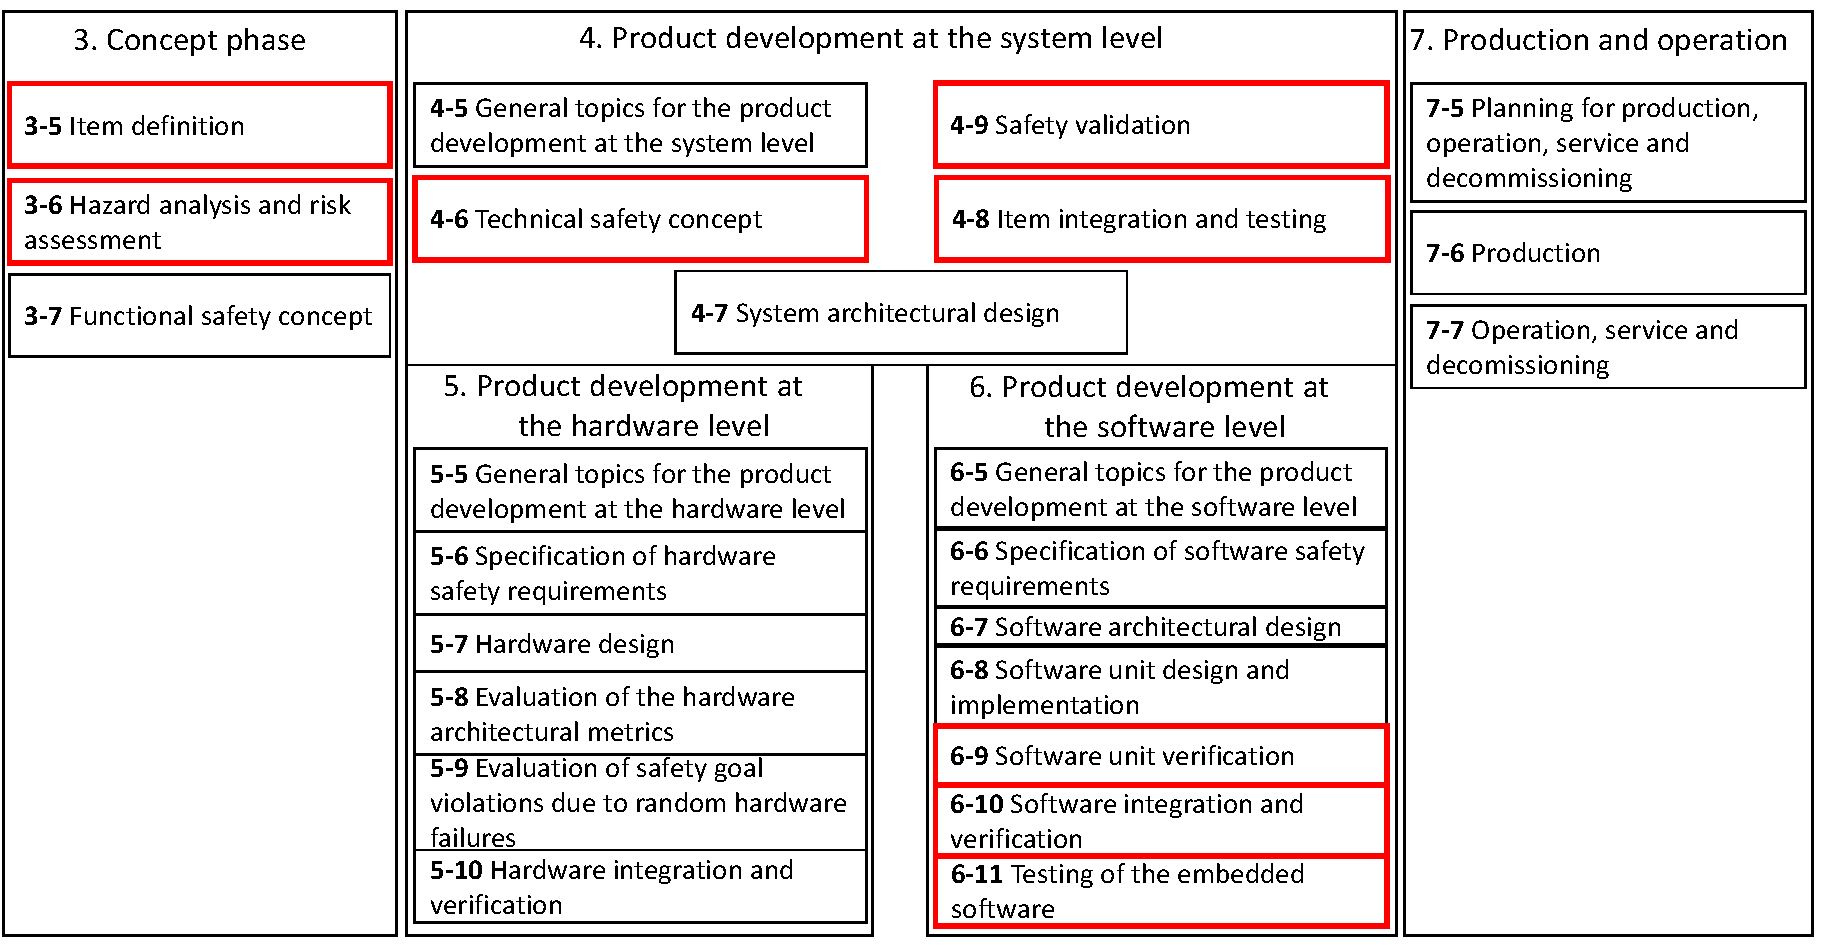
\includegraphics[width=\textwidth]{./3_process/graphics/ISO_Prozess}
	\caption{ISO~26262标准中提出的开发过程概述。红色显示的流程步骤可以利用方案来生成工作产品。}
	\label{fig:ISO-Prozess}
\end{figure*}

\subsection{概念阶段的场景}
%Prior to the technical development, the concept for the item under development is specified.
%During the concept phase of the ISO~26262 standard (part 3) the item is defined, a hazard analysis and risk assessment is conducted, and a functional safety concept is developed.
在标准第3部分的概念阶段,该标准对项目进行了定义,进行了危险分析和风险评估,并引出功能安全概念。

%The item definition shall include a description of the functional concept, system boundaries, the operational environment, the legal requirements, and the dependencies on other items.
项目定义包括功能定义、系统边界、操作环境、法规需求以及对其他项目的依赖关系的描述。基于这些信息,可以派生出可能的操作场景。
%Based on this information, possible operating scenarios can be derived. 
%Reschka \cite{Reschka2016} proposes to identify safe driving states and specify the nominal behavior based on the operating scenarios.
Reschka\cite {Reschka2016}建议识别安全驾驶状态,并根据操作场景指定名义行为。
%The operating scenarios in this process step shall be described in an abstract level of detail and be represented in a human understandable way (textual description).
此过程中的操作场景应以较抽象的方式描述,并以一种易于理解的方式表示。
%The next process step defined by the ISO~26262 standard which uses scenarios is the hazard analysis and risk assessment.
由ISO~26262标准定义的下一个使用场景的过程步骤是危害分析和风险评估。
%The hazard analysis and risk assessment consists of two steps: the situation analysis and the hazard identification, and the classification of hazardous events.
危害分析和风险评估包括两个步骤:情景分析和危险识别,以及危险事件的分类。
%In the situation analysis, all operational situations\footnote{The authors point out that the term `operational situation' as it is used in the ISO~26262 standard should be declared as `operational scenario' according to Ulbrich~et~al.~\cite{ulbrich_definition_2015}.} and operating modes in which malfunctioning behavior will result in a hazardous event shall be described.
在情况分析中,所有操作情况\footnote{作者指出,根据Ulbrich等人的说法,ISO~26262标准中使用的术语“操作情况”应该被称为“操作情景”。 \cite{ulbrich_definition_2015}。}和导致危险事件的故障行为中的操作模式均需要描述。
%Whereby, malfunctioning behavior can be interpreted as deviation from the specified nominal behavior.
%Afterwards, hazardous scenarios, which include a combination of operational scenarios and malfunctioning behavior, will be rated using the automotive safety integrity level (ASIL). 
因此,故障行为可以理解为偏离指定的正常行为。之后,将使用汽车安全完整性等级(ASIL)对危险情景进行评级,其中包括操作情景和故障行为的组合。
%\todo{AR: Geagte These: Ich muss ohnehin alle Szenarien untersuchen, wenn ich es strukturiert und vollständig machen möchte und mich nicht nur auf %Expertenwissen beziehen möchte.}
%The parameters for the ASIL classification are the exposure of the operational scenario, the possible severity, and the controllability of the hazardous scenario\footnote{The controllability of a scenario includes the controllability by the driver/passenger of the automated vehicle and the controllability by other traffic participants.}.
ASIL分类的参数是操作场景的暴露程度,可能的严重程度以及危险场景的可控性\footnote{场景的可控性包括自动驾驶车辆的驾驶员/乘客的可控性以及其他车辆的可控性 交通参与者}。
%In order to determine these parameters, the description of hazardous scenarios has to include the stationary surroundings (scenery) and all traffic participants which may interact with the automated vehicle.
为了确定这些参数,危险场景的描述必须包括静止环境(场景)和可以与自动驾驶车辆交互的所有交通参与者。
%According to the actual state of the art, the analysis of hazardous scenarios is performed by experts. 
%Hence, hazardous scenarios have to be formulated in natural language.
根据现有技术,危险情景的分析由专家进行。因此,必须以自然语言制定危险情景。
%Depending on their area of expertise, human experts vary in the level of detail regarding the terms they use to describe a scenario.
根据他们的专业领域,人类专家在用于描述场景的术语方面的细节水平各不相同。
%Thus, a unified vocabulary for the functional perspective during the process step of the hazard analysis and risk assessment is necessary.
因此,在危害分析和风险评估的过程步骤中,功能视角的统一词汇表是必要的。
%Furthermore, to ensure a common understanding among the experts, the terms within the vocabulary have to be organized in a semi-formal way.
此外,为了确保专家之间的共同理解,词汇表中的术语必须以半正式的方式组织。
%In this way, it is possible to combine vocables from the vocabulary and generate scenarios.
%These scenarios are expressed by language and have a minimal room for interpretation.

%Scenarios have to fulfill the following requirements to be utilized during the concept phase [C] of the ISO~26262 standard:
在ISO~26262标准的概念阶段[C],场景必须满足以下需求:
\begin{itemize}
	\item[C1] 人类专家应该能够用自然语言来描述该场景。
	\item[C2] 场景应以半正式的方式表示。
\end{itemize}


\subsection{系统开发阶段的场景}
%Once the hazardous scenarios have been analyzed, a functional safety concept is developed.
%To implement the functional concept, technical safety requirements have to be derived in process step 4-6.
%As opposed to functional requirements, technical requirements outline criteria which can be physically quantified.
一旦分析了危险场景,就会形成功能安全概念。为了实现功能安全,须提出技术安全需求。与功能需求不同,技术安全需求描述了可量化的条件。
%can be quantified in a physical manner.
%For example, the functional requirement to keep a safe driving distance to other traffic participants can be technically formulated by a distance in meters, which has to be satisfied.
%Hence, every hazardous scenario has to be converted from the linguistic and semi-formal representation of the \textit{concept phase} to a representation via state values for the technical \textit{product development on system level} (4).
例如,保持与其他交通参与者的安全驾驶距离的安全需求通过以米为单位的距离来确定。因此,每个危险场景都必须从半正式的自然语言表述(概念阶段)转换为利用状态量表述(系统开发阶段)的方式。
%A list of those state variables is a precise description of a scenario, but, due to the high level of detail, not intuitively processable by human experts.
这些状态量的列表是对场景的精确描述,但由于细节水平抽象程度高,人类专家无法直观地处理这些状态量。
%To reduce the quantity of scenarios, state values can be summarized in value ranges. 
%Later on, those value ranges can be further detailed in valid/invalid ranges to define a set of safe and unsafe values respectively, or to model the system boundaries.
为了减少场景的数量,可以给定状态量的取值范围,或者可以进一步划分有效/无效的取值范围,即安全/不安全的取值,从而明确系统边界。场景的详细表述确保了能以可验证的方式制定开发项目的需求。
%A detailed representation of scenarios ensures that the requirements on the item to be developed can be formulated in a verifiable way.
方案的详细表述确保了可以以可验证的方式制定对待开发项目的需求。
%This is a necessary condition for the safety validation in process step 4-9 of the ISO~26262 standard.
这是ISO~26262标准的步骤4-9中的安全验证的必要条件。
%All in all, scenarios have to fulfill the following requirements to be utilized during the system development phase [S] of the ISO~26262 standard:
总而言之,场景必须满足ISO~26262标准的系统开发阶段[S]中要使用的以下需求:
\begin{itemize}
	\item[S1] 场景应包括用于场景表示的状态量的参数范围。
	\item[S2] 场景应为每项参数指定一个标记,以支持自动处理。
\end{itemize}

\subsection{测试与验证阶段的场景}
%During the test phase, it is examined whether the implemented system fulfills the requirements specified in the previous process steps.
在测试阶段,将验证系统是否满足了前述流程中指定的需求。
%For this verification, the tests have to be systematically planned, specified, executed, evaluated, and documented \cite[part 8, section 9.2]{ISO_26262_2011}.
这一过程,验证必须依据标准\cite[part 8, section 9.2]{ISO_26262_2011},系统地计划、制定、执行、评估和记录。
%Each test case specification has to include the following information independently from the test method \cite[part 8, section 9.4.2]{ISO_26262_2011}:
每个测试用例规范必须独立于测试方法包括以下信息\cite[part 8, section 9.4.2]{ISO_26262_2011}:
\begin{enumerate}
\item  一个独特的标识
\item 要验证的工作产品的引用参考
\item 前提条件和配置\footnote{在系统变体的意义上。}
\item 环境条件
\item 输入数据,包括它们的时间顺序
\item 预期的行为,包括可接受的变化
\end{enumerate}

%A very challenging aspect of the test case generation is the specification of input data.
测试用例生成的一个难点在于输入数据的规范性,包括每个参数的时间序列,这些时间序列实质上影响测试对象的行为。
%This data has to include time sequences of each parameter which is essentially affecting the behavior of the test object.
%At the same time, due to highly connected systems, the input data may not contain any inconsistencies\footnote{Unintended inconsistencies are meant here. Fault injections can be utilized as a test method later on.}, but rather represent a consistent scenario.
同时,由于高度连接的系统,输入数据可能不包含任何不一致\footnote{这里不一致的意思:故障注入可以在以后用作测试方法。},而是代表一致的场景。
%Information regarding the operational environment of the system under verification as well as possible operating scenarios are already given in the item definition, which is specified during the concept phase of the development process according to the ISO~26262 standard.  
概念阶段已经给出了系统的操作环境和可能的操作场景,这是为测试用例派生一致的输入数据的基础
%Based on this information, consistent input data can be derived for the specification of test cases.
%The scenarios used in the item definition are expressed by language and formulated on an abstract level of detail. 
项目定义中使用的场景由语言表达,并在抽象的详细程度上制定。
%To utilize these abstract scenarios within the scope of a test case, the scenarios have to be specified in detail and concretized.
要在测试用例的范围内使用这些抽象场景,必须详细指定场景并使其具体化。
%The detailed specification of scenarios can be performed within the scope of the \textit{specification of technical safety requirements} \cite[part 4, section 6]{ISO_26262_2011}.
场景的详细规范可以在技术安全需求规范的范围内进行\cite[part 4, section 6]{ISO_26262_2011}.
%The technical safety requirements describe how the item has to react to external stimuli which can affect the compliance with the safety goals.
技术安全要求描述了项目如何对可能影响安全目标的外部影响做出反应。
%The technical requirements specify the linguistic requirements 
%In this way, the technical requirements also define for which parameter ranges the functionality of the system under development has to be ensured.
通过这种方式,技术要求还定义了必须确保正在开发系统的功能参数范围。
%This parameter space has to be tested during the verification process and thus has to be taken into account for the test case generation.
必须在验证过程中测试该参数空间,因此必须考虑该生成测试用例。
%In addition, the scenarios have to be converted to a formal representation during the step of specifying the scenarios in detail.
%A formal representation is necessary, to ensure a reproducible test case execution later on.
此外,还必须将场景转换为正式表达,以确保之后测试用例的可执行性及可复现性。
%To ensure a reproducible test case execution later on, a formal representation is necessary.
%The scenarios have to define all parameters required for test case execution via different test methods (like simulation or field tests).
场景必须通过不同的测试方法(如模拟或现场测试)定义测试用例执行所需的所有参数。
%Thus, in the step of specifying a scenario in detail, a conversion has to be conducted from an informal description based on organized terms to a formal description based on physical system state values.
因此,在详细指定场景的步骤中,必须从基于有组织的术语的非正式描述到基于物理系统状态值的形式描述进行转换。
%To generate the input data included in a test case, discrete parameter values have to be chosen from the continuous parameter ranges of a specified scenario in a concretization step.
为了生成测试用例的输入数据,必须从指定场景的连续参数范围中选择离散参数值。
%Schuldt \cite{Schuldt2017} proposes the use of equivalence classes, boundary value analysis, and combinatorial methods for identifying representative samples.
Schuldt \cite{Schuldt2017}提出使用等价类,边界值分析和组合方法来识别代表性样本。
%This approach provides a systematic generation of test cases, but lacks a method to determine a meaningful test coverage.
这种方法提供了系统生成的测试用例,但缺乏确定有意义的测试覆盖率的方法。
%For determining a meaningful test coverage, the test concept, the scenario selection, and the necessary test methods have to be taken into account.
为了确定有意义的测试覆盖率,必须考虑测试概念,场景选择和必要的测试方法。
%The scenarios, which are systematically derived during the concretization step and then formally described, represent consistent input data for the item under test.
在具体步骤中系统地导出,然后正式描述的场景代表被测系统的一致输入数据。
%Thus, the derived scenarios can be used in the scope of a test case for the verification of the implemented system.
因此,派生的场景可以在测试用例的范围内用于验证所实现的系统。
%All in all, scenarios have to fulfill the following requirements to be utilized during the testing phase [T] of the ISO~26262 standard:
总而言之,场景必须满足ISO~26262标准的测试阶段[T]中要使用的以下要求:

\begin{itemize}
	\item[T1] 场景应该通过具体的状态值来描述,以确保其可执行性和可复现性。
	\item[T2] 场景应具备一致性。
	\item[T3] 场景应该以一种高效的机器可读的方式表示,以确保自动化测试的执行。
\end{itemize}

\subsection{对场景需求的分析}
%Table \ref{tab:contradictoryRequirements} illustrates that the specified requirements are contradictory regarding the form of scenario description. 
表\ref {tab:contradictoryRequirements}说明了指定的要求与场景描述的矛盾。
%On the one hand, requirement C1 states the demand for an abstract, linguistic scenario representation and, on the other hand, requirements S2 and T3 state the demand for an efficient, machine readable scenario representation.
一方面,需求概念阶段C1表示对抽象的语言场景表示的需求,另一方面,需求S2和T3表示对有效的机器可读场景表示的需求。
%Since linguistic representations are hard to process by machines and human beings are not able to read size efficient (mostly binary coded) data formats, there is a demand for different forms of scenario representations.
由于语言表示很难由机器处理,并且人类无法读取大小有效(主要是二进制编码)的数据格式,因此需要不同形式的场景表示。
%Similarly, requirements S1 and T2 demand different levels of detail for the scenario representation.
类似地,S1和T2场景需求表示的不同细节程度。
%On the one hand, requirement S1 asks for a scenario representation via parameter ranges in the state space. 
一方面,需求S1通过状态空间中的参数范围来表述场景。
%This form of representation offers multiple degrees of freedom regarding the determination of concrete values to be tested.
这种表示形式在确定要测试的具体值方面提供了多个自由度。
%On the other hand, requirement T2 asks for a representation that includes concrete parameter values. 
另一方面,需求T2要求包括具体参数值来表述需求。
%This form of representation is required for a reproducible test case execution.
这是测试用例可重复执行的必要条件
%Hence, machine readable scenarios have to support two different levels of detail.
因此,机器可读的场景必须支持两种不同的细节程度。

\begin{table*}
	\centering
	\caption{场景需求的矛盾 ($\perp$ 矛盾标记)}
	\label{tab:contradictoryRequirements}
	\begin{tabularx}{\textwidth}{ X l X l X }
		\hline \\
		概念阶段 & & 系统开发阶段 & & 测试阶段 \\
		\hline \\
	人类专家应能够用自然语言制定该领域的术语。 & \multirow{3}{4pt}{$\perp$} &  场景应包括用于场景表述的状态值的参数范围。 & \multirow{3}{4pt}{$\perp$} & 场景应通过具体的状态值建模,以确保其可重复性并能够使测试方法执行场景。 \\
		\hline \\
	\end{tabularx}
\end{table*}

\section{设计和测试过程中的场景术语}
\label{terminologie}
%
%As stated in the previous section, the requirements on the type of scenario representations in the development process of the ISO~26262 standard are contradictory.
正如上一节所述,在ISO 26262标准的开发过程中应用场景时,对场景的细节程度的需求是存在矛盾的。
%In the following section, the authors will suggest three abstraction levels for scenarios and show how these abstraction levels can be converted into each other along the development process.
在下一节中,作者将为场景建议三个抽象级别,并展示如何在开发过程中将这些抽象级别相互转换。
%Fig. \ref{fig:Abstraktionsebenen} illustrates the three levels of abstraction for scenarios: \textit{functional scenarios}, \textit{logical scenarios}, and \textit{concrete scenarios}.
作者将场景划分为三个抽象级别:功能场景(Functional scenarios)、逻辑场景(Logical scenarios)和具体场景(Concrete scenarios),如图\ref{fig:Abstraktionsebenen}所示。

\begin{figure*}
	\centering
	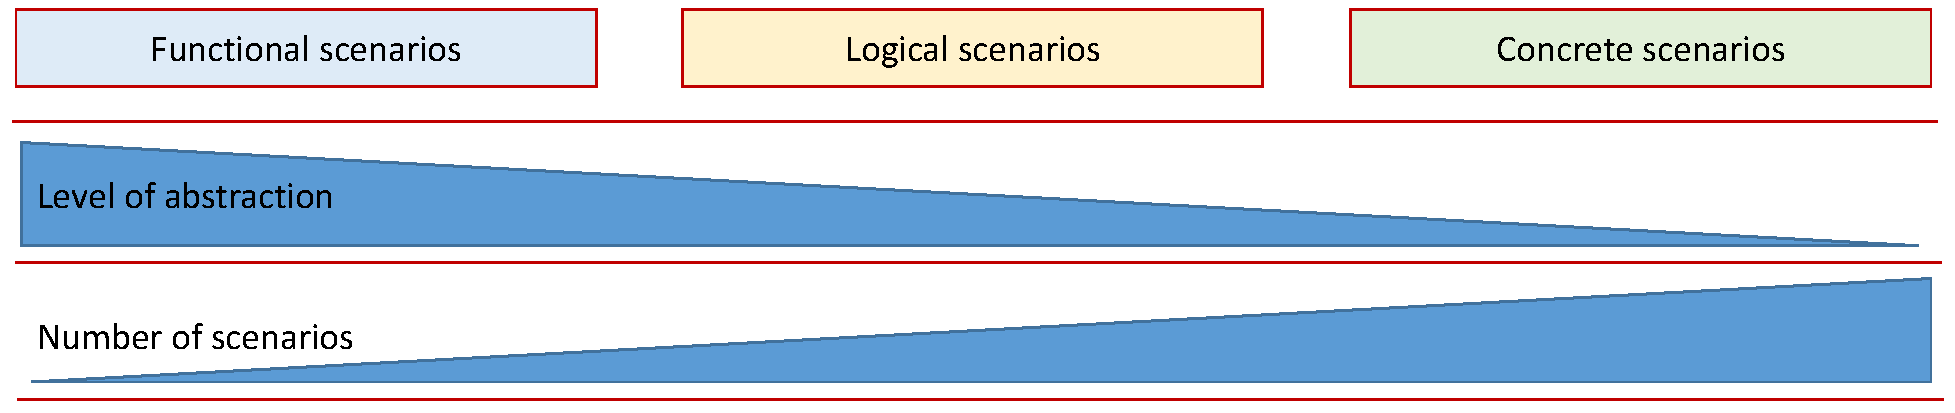
\includegraphics[width=1.0\textwidth]{./4_terminology/graphics/Abstraktionsebenen_reduziert2}
	\caption{ISO~26262标准开发过程中的抽象程度}
	\label{fig:Abstraktionsebenen}
\end{figure*}

\subsection{功能场景}
%Functional scenarios depict the most abstract level of scenario representations.
功能场景是场景表述的最抽象级别。
%These scenarios may be used for the item definition and the hazard analysis and risk assessment during the concept phase of the ISO~26262 standard.
在概念阶段,这些场景可用于项目定义、危险分析和风险评估。
%They are represented by language to ensure that human experts can easily understand existing scenarios, discuss them, and create new scenarios. 
它们以语言表示,以确保人类专家可以轻松理解现有场景,讨论它们并创建新场景。
%The authors suggest the following definition:
作者提出了以下定义:
\begin{quote}
\textit{
%Functional scenarios include operating scenarios on a semantic level.
功能场景包括语义级别的操作场景。
%The entities of the domain and the relations of those entities are described via a linguistic scenario notation.
通过语言场景符号来描述域内的实体以及实体间的关系。
%The scenarios are consistent.
场景是一致的。
%The vocabulary used for the description of functional scenarios is specific for the use case and the domain and can feature different levels of detail.
用于描述功能场景的术语表应由一般用例或域内专用的术语组成,并且可以具有不同的详细程度。
}
\end{quote}

%The representation of functional scenarios on a semantic level includes a linguistic and consistent description of entities and relations/interactions of those entities.
%For the linguistic description a consistent vocabulary has to be defined.
%This vocabulary includes terms for different entities (vehicle A, vehicle B) and phrases for the relations of those entities (vehicle A overtakes vehicle B). 
功能场景的表述包括实体和实体之间的关系,不同场景的描述方式必须是一致的。首先需要制定一个术语表,这个术语表包括不同实体的术语(车辆A、车辆B)和这些实体的关系短语(车辆A超越车辆B)。 

%The required level of detail of functional scenarios depends on the actual development phase and the item under development.
%Both aspects must be considered during the definition of the vocabulary.
功能方案所需的详细程度取决于实际开发阶段和正在开发的项目。在词术语表的定义过程中必须考虑这两个方面。
%For example, a highway pilot requires a vocabulary to describe the road geometry and topology, interactions with other traffic participants, and weather conditions. 
例如,高速公路飞行员需要术语表来描述道路几何形状和拓扑结构,与其他交通参与者的交互以及天气状况。
%On the contrary, a parking garage pilot requires a vocabulary to describe the layout of the building whereas weather conditions may be irrelevant.
相反,停车库行驶需要术语表来描述建筑物的布局,而天气条件可能是无关紧要的。
%If a comprehensive vocabulary is used for the description of the entities and the relations of those entities, a large amount of scenarios can be derived from the vocabulary.
如果使用综合术语表来描述实体和这些实体的关系,则可以从术语表中导出大量场景。
%For a generation of consistent functional scenarios, all terms of the vocabulary have to be distinct.
对于一致的功能场景泛化,术语表的所有术语必须是不同的。
%Sources for terms that define the entities of a domain are, for example, actual standards and guidelines like road traffic regulations or the German standard for constructing motorways
定义域实体的术语来源是,例如,道路交通法规或德国高速公路建设标准等实际标准和指南\cite{RAA}。

\begin{figure}
	\centering
	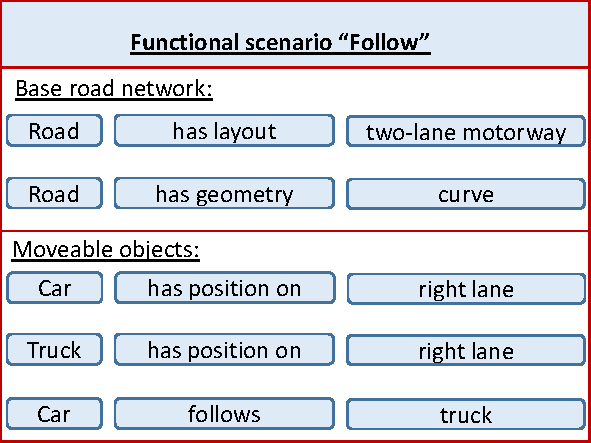
\includegraphics[width=0.9\columnwidth]{./4_terminology/graphics/functionalScenario.pdf}
	\caption{在高速公路行驶的一个功能场景:一辆轿车和一辆卡车正行驶在右侧车道上,轿车跟随卡车行驶。}
	\label{fig:functionalScenario}
\end{figure}

%Fig. \ref{fig:functionalScenario} shows a functional scenario for a highway pilot on a two-lane motorway in a curve.
%A car and a truck are driving on the right lane of the road, whereby the car follows the truck.
%In this example, the road is described with a layout and a geometry.
图\ref{fig:functionalScenario}为在高速公路行驶的一个功能场景:一辆轿车和一辆卡车正行驶在右侧车道上,轿车跟随卡车行驶。在这个例子中,道路特征主要描述为横断面布置情况和几何结构特征。
%Depending on the item's use case and domain, the vocabulary has to include additional terms to describe these characteristics like `three-lane motorway' for layout, and `straight' or `clothoid' for geometry.
根据项目的用例和域,词汇表必须包含用于描述这些特征的附加术语,例如用于布局的“三车道高速公路”,以及用于几何的“直线”或“回旋曲线”。
%The scenario can be varied by choosing other terms from the defined vocabulary.
通过从定义的术语表中选择其他术语,可以改变场景。
\subsection{逻辑场景}
%Logical scenarios depict a detailed representation of functional scenarios with the help of state space variables.
基于状态空间变量,逻辑场景是对功能场景的进一步详细描述。
%Hence, functional scenarios can be converted into a representation which is based on parameters. 
%Those state space variables describe the entities and the relations of those entities.
那些状态空间变量描述了这些实体的实体和关系。
%Logical scenarios may be used to derive and represent requirements for the item during the system development phase.
在系统开发阶段,可以利用逻辑场景派生出安全需求。
%For that purpose, logical scenarios describe the value ranges of the state space variables via a formal notation.
为此,逻辑场景通过正式表示法描述状态空间变量的值范围。
%The authors suggest the following definition for logical scenarios:
作者提出了以下定义:
\begin{quote}
\textit{
%Logical scenarios include operating scenarios on a state space level.
%Logical scenarios represent the entities and the relations of those entities with the help of parameter ranges in the state space.
%The parameter ranges can optionally be specified with probability distributions.
%Additionally, the relations of the parameter ranges can optionally be specified with the help of correlations or numeric conditions.
%A logical scenario includes a formal notation of the scenario.
逻辑场景以状态空间呈现操作场景。通过定义状态空间内变量的参数范围,可以表达实体特征和实体间的关系。参数范围可以选择用概率分布来确定。此外,不同参数的关系可以通过相关性或数值条件来确定。逻辑场景应包含该场景的形式标记。
}
\end{quote}

%The logical scenario description covers all elements necessary for the derivation of technical requirements needed to implement a system which solves these scenarios.
逻辑场景涵盖了提出安全需求所需的所有元素。
%For a step-wise specification of scenarios in the development process of the ISO~26262 standard, logical scenarios have to be described via a formal notation in the state space, whereby parameters have to be defined via value ranges.
为了在标准规定的开发过程中逐步规范场景,必须在状态空间中通过形式标记来表述逻辑场景,并从取值范围中确定参数。
%the linguistic representation of functional scenarios has to be converted to the formal state space notation of logical scenarios.  
%The state space of logical scenarios is described via parameters and value ranges for those parameters.
%For a more detailed description of those parameter ranges, probability distributions (e.g., Gaussian distribution, Uniform distribution) can optionally be specified for each parameter range.
可以通过概率分布(例如,高斯分布,均匀分布)为每个参数指定范围。
%Additionally, relations of the parameter ranges can optionally be specified by numeric conditions (e.g., the speed of an overtaking vehicle has to be greater than the speed of the overtaken vehicle) or correlation functions (e.g., lane width correlates with curve radius).
参数范围间的关系可以由数值条件或相关函数来指定(例如,超车速度必须大于被超车速度,车道宽度与曲线半径相关)。

\begin{figure}
	\centering
	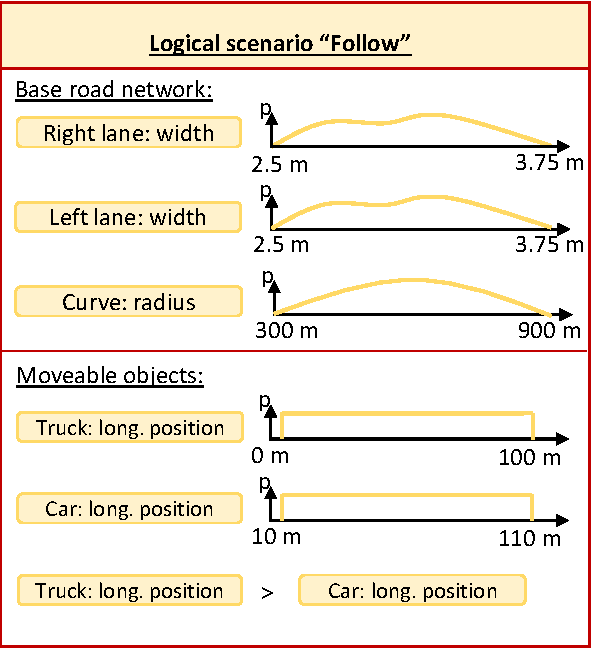
\includegraphics[width=0.9\columnwidth]{./4_terminology/graphics/logicalScenario.pdf}
	\caption{逻辑场景的示例。 一辆汽车沿着双车道高速公路右侧车道的一辆卡车行驶。}
	\label{fig:logicalScenario}
\end{figure}

%Fig. \ref{fig:logicalScenario} shows a logical scenario that has been derived from the functional scenario illustrated in Fig. \ref{fig:functionalScenario}.
图\ref{fig:logicalScenario}显示了从图\ref{fig:functionalScenario}所示的功能场景中衍生出的逻辑场景。
%Functional scenarios are converted to logical scenarios by a transformation from the linguistic representation into state space and specification of the scenario describing parameters.
通过从语言表述到状态空间的转换以及描述参数的场景的规范,功能场景被转换为逻辑场景。
%Hence, every term from the vocabulary has to be assigned to parameters which describe this term.
因此,功能场景术语表中的每一项都必须分配一个描述该术语的参数。
%In this example, both lanes are described via a lane width, the curve geometry is represented by a radius, and the vehicles are described by longitudinal positions along the lane.
%Furthermore, the term `follows' demands that the longitudinal position of the truck is greater than the longitudinal position of the car.
在这个例子中,两条车道都是通过车道宽度来描述的,几何结构是由一个半径来表示的,车辆由其纵向位置来描述,并要求卡车纵向位置大于轿车。本文作者选择了一组简化的参数。在实际应用中,可能需要多个参数来描述单个术语,例如,一辆卡车可以通过规定其尺寸、重量和发动机功率来定义。
%To allow the example to be reflected in this paper, the authors have chosen a reduced set of parameters.
%
%%Hence, the example can be handled in this paper, the authors have chosen a very narrow parameter space.
%In reality, much more parameters will be necessary to describe a single term from the vocabulary.
%%In reality there will be much more parameters necessary to describe a single term from the vocabulary.
%For example, a truck can additionally be specified by its dimensions, weight, and engine power.

%In addition, for every parameter from the example in Fig.~\ref{fig:logicalScenario} the value range and the probability distribution, with which the parameter occurs in reality, are specified.
另外,对于图~\ref {fig:logicalScenario}中的示例的每个参数,指定了值范围和参数实际出现的概率分布。
%This information helps to formulate technical requirements in the system development phase and provide a basis for a systematic generation of concrete scenarios in the testing phase.
该信息有助于在系统开发阶段制定技术要求,并为在测试阶段系统生成具体方案提供基础。

%
%\todo{Logical scenarios are scenarios, which describe an episode of traffic on a semi-formal level. The scenario description covers all elements necessary for the derivation of technical requirements to implement a system, which solves these scenarios. Logical scenarios include parameter descriptions and ranges for all elements of the scenario, including related probability distributions of parameter values.}
%\todo{AR: Enthalten logische Szenarien auch Informationen über die Beziehungen zwischen Elementen des Szenarios oder nicht? Z.B.: Tempolimit für Fahrstreifen versus Fahrstreifen und Schild ohne Beziehung zueinander?}
%\todo{AR: Folgenden Satz würde ich nach der Definition anhängen, da er ja nicht teil der Definition ist: The parameter space and the value ranges can be derived from the abstract linguistic representaion of functional scenarios and have to be defined distinctly.}

\subsection{具体场景}
%Concrete scenarios describe the entities and the relations for those entities using distinct parameters in the state space.
具体场景由某个确定的参数值来表示状态空间中实体和实体间关系
%Every logical scenario can be converted to a concrete scenario by selection of a concrete value from a parameter range.
每个逻辑场景都可以通过从参数范围中选择具体值来转换为具体场景。
%Concrete scenarios may be used as a basis for test case generation in the testing phase.
具体场景可以作为测试用例的基础。作者提出了以下定义:
%The authors suggest the following definition for concrete scenarios:

\begin{quote}
\textit{
%Concrete scenarios distinctly depict operating scenarios on a state space level.
%Concrete scenarios represent entities and the relations of those entities with the help of concrete values for each parameter in the state space.
具体场景以状态空间详细描述了操作场景。通过确定状态空间中每个参数的具体值来明确描述实体和实体间的关系。
}
\end{quote}

%For each logical scenario with continuous value ranges any number of concrete scenarios can be derived.
对于每一个具有连续取值范围的逻辑场景,都可以派生出任意数量的具体场景。
%For example, an infinite number of concrete scenarios can be achieved by choosing an infinitesimal sampling step width for each parameter.
例如,通过为每个参数选择无穷小的采样步长,可以实现无限数量的具体场景。
%An efficient concretization is accomplished by identification and combination of representative discrete values for each parameter.
为保证生成具体场景的效率,应选择有代表性的离散值进行组合。
%Only concrete scenarios can directly be converted into test cases and executed with a vehicle guidance system.
必须强调的是,只有具体场景可以直接转化为测试用例。

\begin{figure}
	\centering
	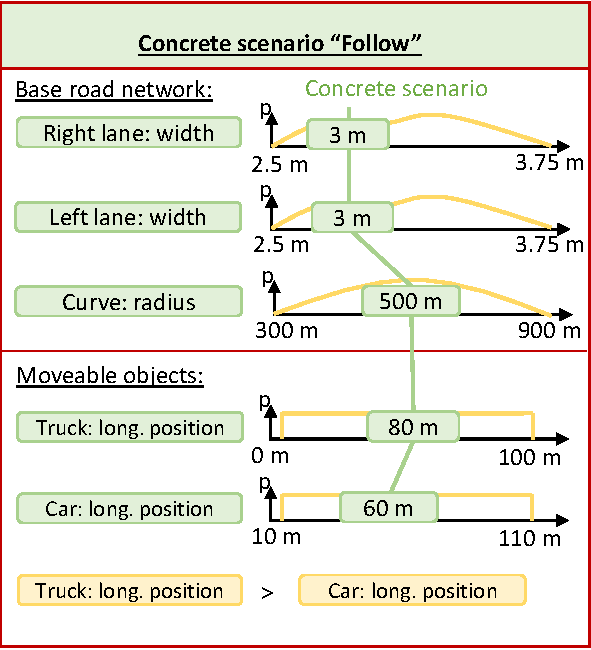
\includegraphics[width=0.9\columnwidth]{./4_terminology/graphics/concreteScenario.pdf}
	\caption{具体场景示例。一辆汽车沿着双车道高速公路右侧车道的一辆卡车行驶。}
	\label{fig:concreteScenario}
\end{figure}

%Fig. \ref{fig:concreteScenario} shows a concrete scenario that has been derived from the logical scenario illustrated in Fig. \ref{fig:logicalScenario}.
图\ref{fig:concreteScenario}为一个具体的场景,该场景由图\ref{fig:logicalScenario}中所示的逻辑场景衍生。
%For every parameter, a concrete value within the value range has been chosen.
%Logical scenarios are converted to concrete scenarios by choosing a concrete value within the value range for each parameter.
%For every parameter a concrete value within the defined value range has been chosen while the specified condition regarding the parameters has been satisfied.
对于每个参数,已经选择了在定义的值范围内的具体值,同时满足了关于参数的指定条件。
%To transform concrete scenarios into test cases, concrete scenarios have to be augmented by the expected behavior of the test object and the test infrastructure to be used as stated by Ulbrich~et~al.~\cite{ulbrich_definition_2015}.
%The expected behavior can be derived from the functional operating scenarios, the logical scenarios, or the item definition. 
要将具体场景转换成测试用例,需要增加被测对象的预期行为表现,以及对相关测试设施的需求~\cite{ulbrich_definition_2015}。而被测对象的预期行为则可以从操作场景、逻辑场景或项目定义中导出。
%
%\subsection{Integration of the scenario definitions into the development process}
%
%\begin{figure*}[b!]
%	\centering
%	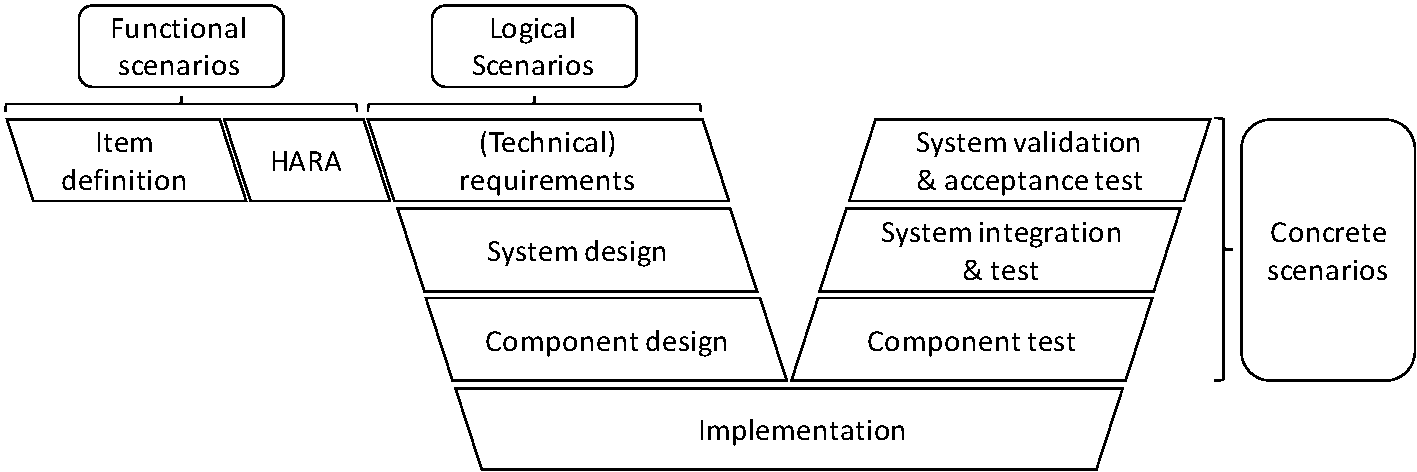
\includegraphics[width=0.75\textwidth]{./4_terminology/graphics/V_Modell}
%	\caption{Functional, logical and concrete scenarios in the V-model-based development process; HARA: Hazard analysis and risk assessment}
%	\label{fig:Prozess}
%\end{figure*}

%
%In the concept phase, functional scenarios are used to define the operating scenarios of the item and build a basis for a hazard analysis and risk assessment.
%To enable human experts to discuss about occurring risks, functional scenarios are represented in a linguistic way.

%Functional, logical, and concrete scenarios can be converted into each other.
%Functional scenarios can be converted to logical scenarios by a transformation from the linguistic representation into state space and specification of the scenario describing parameters.
%Logical scenarios can be converted to concrete scenarios by concretization of each parameter range to a concrete value.
%Fig. \ref{fig:Prozess} shows a schematic development process based on the V-model with the suggested levels of scenario abstraction.
%
%Before the technical development starts, functional scenarios are used for the item definition and the hazard analysis and risk assessment.
%Functional scenarios are represented linguistically and have to be converted to logical scenarios by a transformation into the state space and specification of the scenario describing parameters.
%Within this context, technical requirements can be formulated by valid and invalid value ranges of the parameters describing the scenario respectively.
%
%
%Concrete scenarios are the basis for executable test cases.
%A test case contains a concrete scenario and additionally the pass/fail criteria, which result from the desired behavior of the system under test. In logical scenarios, the possible parameters of all movable objects are available in the parameter ranges. Thus, the desired behavior of the ego vehicle can't be derived in general, since it is different for specific parameter sets.
%To transform concrete scenarios into test cases, concrete scenarios have to be augmented by the expected behavior of the test object and the test infrastructure to be used as stated by Ulbrich~et~al.~\cite{ulbrich_definition_2015}.
%The expected behavior can be derived from the functional operating scenarios, the logical scenarios, or the item definition. 
%
%A big difference of concrete scenarios and test cases is the representation of the behavior of the test object.
%Within a test case, the resulting behavior of the test object is not known. The resulting behavior first occurs, when the test case is executed.
%In concrete scenarios the behavior of all traffic participants is at least known by their goals and values.





\section{结论与展望}
\label{conclusion}
%In this paper, the authors analyzed the practicability of a scenario-based approach for the design of vehicle guidance systems following the development process of the ISO 26262 standard.
本文分析了基于场景的方法在依据ISO 26262标准开发自动驾驶系统过程中的可行性。
%analyzed the development process of the ISO~26262 standard regarding the practicability of a scenario-based development for vehicle guidance systems.
%For this purpose, the process steps in which scenarios may be used to generate the work products of the respective process step have been identified.
%Furthermore, requirements regarding the representation of scenarios have been defined and contradictions regarding the requirements resulting from different process steps have been shown.
作者分析了可以使用场景来生成工作输出产品的各个工作阶段,并明确了不同阶段对场景描述的需求,阐述了场景描述需求在细节程度上存在的差异。
%On this basis, the authors suggested three levels of abstraction for scenarios in order to fulfill all requirements defined above.
在此基础上,作者定义了场景的三个抽象级别,以满足上文阐述的场景需求。
%Furthermore, a definition for each introduced level of abstraction has been given and it has been shown, how the levels of abstraction for scenarios can be used to generate work products for different process steps defined in the ISO~26262 standard.
此外,作者给出了每个抽象级别的定义,并说明了如何使用场景的抽象级别来生成ISO~26262标准中定义的不同阶段的工作产品。
%In the future, new methods and tools are needed to generate functional scenarios and to convert these functional scenarios to concrete scenarios along the development process of the ISO~26262 standard. 
未来,需要新的方法和工具来生成功能场景,并将这些功能场景转换为ISO~26262标准开发过程中的具体场景。
%In addition to this contribution, there is a companion contribution submitted to the 2018 IEEE Intelligent Vehicles Symposium with an knowledge based approach for creating functional scenarios with a large variety.
除了这一贡献之外,还提交了2018年IEEE智能车辆研讨会的配套文稿,其中提供了基于知识的方法,用于创建各种各样的功能场景。
%Therefore, existing data formats for scenarios can be integrated into the suggested levels of abstraction.
因此,场景的现有数据格式可以集成到建议的抽象级别中。
%Afterwards, new methods and tools for scenario specification and scenario concretization can be developed with respect to a test concept for automated vehicles.
之后,可以针对自动驾驶车辆的测试概念,开发用于场景规范和场景具体化的新方法和工具。


\bibliographystyle{IEEEtran}
%\bibliography{bib/bib}
\begin{thebibliography}{10}
	\providecommand{\url}[1]{#1}
	\csname url@samestyle\endcsname
	\providecommand{\newblock}{\relax}
	\providecommand{\bibinfo}[2]{#2}
	\providecommand{\BIBentrySTDinterwordspacing}{\spaceskip=0pt\relax}
	\providecommand{\BIBentryALTinterwordstretchfactor}{4}
	\providecommand{\BIBentryALTinterwordspacing}{\spaceskip=\fontdimen2\font plus
		\BIBentryALTinterwordstretchfactor\fontdimen3\font minus
		\fontdimen4\font\relax}
	\providecommand{\BIBforeignlanguage}[2]{{%
			\expandafter\ifx\csname l@#1\endcsname\relax
			\typeout{** WARNING: IEEEtran.bst: No hyphenation pattern has been}%
			\typeout{** loaded for the language `#1'. Using the pattern for}%
			\typeout{** the default language instead.}%
			\else
			\language=\csname l@#1\endcsname
			\fi
			#2}}
	\providecommand{\BIBdecl}{\relax}
	\BIBdecl
	
	\bibitem{SAE2016}
	{Society of Automotive Engineers (SAE)}, ``J3016 - {Taxonomy and Definitions
		for Terms Related to On-Road Motor Vehicle Automated Driving Systems},''
	{Society of Automotive Engineers (SAE)}, 2016.
	
	\bibitem{noauthor_techday_nodate}
	\BIBentryALTinterwordspacing
	``\BIBforeignlanguage{en}{{TechDay} piloted driving -- {The} traffic jam pilot
		in the new {Audi} {A}8},'' 2017, accessed: 01--15--2018. [Online]. Available:
	\url{https://www.audi-mediacenter.com/en/techday-piloted-driving-the-traffic-jam-pilot-in-the-new-audi-a8-9276}
	\BIBentrySTDinterwordspacing
	
	\bibitem{hawkins_waymo_2017}
	\BIBentryALTinterwordspacing
	``Waymo is first to put fully self-driving cars on {US} roads without a safety
	driver,'' 2017, accessed: 01--15--2018. [Online]. Available:
	\url{https://www.theverge.com/2017/11/7/16615290/waymo-self-driving-safety-driver-chandler-autonomous}
	\BIBentrySTDinterwordspacing
	
	\bibitem{wachenfeld_release_2016}
	W.~Wachenfeld and H.~Winner, ``\BIBforeignlanguage{en}{The {Release} of
		{Autonomous} {Vehicles}},'' in \emph{\BIBforeignlanguage{en}{Autonomous
			{Driving}}}, M.~Maurer, J.~C. Gerdes, B.~Lenz, and H.~Winner, Eds.\hskip 1em
	plus 0.5em minus 0.4em\relax Berlin, Heidelberg, Germany: Springer Berlin
	Heidelberg, 2016, pp. 425--449.
	
	\bibitem{ulbrich_definition_2015}
	S.~Ulbrich, T.~Menzel, A.~Reschka, F.~Schuldt, and M.~Maurer, ``{Defining and
		Substantiating the Terms Scene, Situation, and Scenario for Automated
		Driving},'' in \emph{2015 {IEEE} 18th {International} {Conference} on
		{Intelligent} {Transportation} {Systems} ({ITSC})}, Las Palmas, Spain, 2015,
	pp. 982--988.
	
	\bibitem{SzenarienProzess2017}
	G.~Bagschik, T.~Menzel, A.~Reschka, and M.~Maurer, ``{Szenarien
		Entwicklung, Absicherung und Test von automatisierten Fahrfunktionen -
		English title: Scenarios for Development, Test and Validation of Automated
		Vehicles},'' in \emph{11. {Workshop} {Fahrerassistenz und automatisiertes
			Fahren} {FAS} 2017}, Walting, Germany, 2017.
	
	\bibitem{go_blind_2004}
	K.~Go and J.~M. Carroll, ``The {Blind} {Men} and the {Elephant}: {Views} of
	{Scenario}-based {System} {Design},'' \emph{Interactions}, vol.~11, no.~6,
	pp. 44--53, 2004.
	
	\bibitem{bergenhem_how_2015}
	C.~Bergenhem, R.~Johansson, A.~S\"oderberg, J.~Nilsson, J.~Tryggvesson,
	M.~T\"orngren, and S.~Ursing, ``How to {Reach} {Complete} {Safety}
	{Requirement} {Refinement} for {Autonomous} {Vehicles},'' in \emph{{CARS}
		2015-{Critical} {Automotive} applications: {Robustness} \& {Safety}}, Paris,
	France, 2015.
	
	\bibitem{bagschik_identification_2016}
	G.~Bagschik, A.~Reschka, T.~Stolte, and M.~Maurer, ``Identification of
	{P}otential {H}azardous {E}vents for an {Unmanned} {Protective} {Vehicle},''
	in \emph{2016 {IEEE} {Intelligent} {Vehicles} {Symposium} ({IV})},
	Gothenburg, Sweden, 2016, pp. 691--697.
	
	\bibitem{stolte_towards_2015}
	T.~Stolte, A.~Reschka, G.~Bagschik, and M.~Maurer, ``Towards {Automated}
	{Driving}: {Unmanned} {Protective} {Vehicle} for {Highway} {Hard} {Shoulder}
	{Road} {Works},'' in \emph{2015 {IEEE} 18th {International} {Conference} on
		{Intelligent} {Transportation} {Systems} ({ITSC})}, Las Palmas, Spain, 2015,
	pp. 672--677.
	
	\bibitem{schuldt2011}
	F.~Schuldt, F.~Saust, B.~Lichte, M.~Maurer, and S.~Scholz, ``{Effiziente
		systematische Testgenerierung f\"ur Fahrerassistenzsysteme in virtuellen
		Umgebungen - English title: Efficient systematic test case generation for
		automated driving functions in virtual driving environments},'' in \emph{AAET
		- Automatisierungssysteme, Assistenzsysteme und eingebettete Systeme
		Transportmittel}, Braunschweig, Germany, 2013, pp. 114 -- 134.
	
	\bibitem{bach_model_2016}
	J.~Bach, S.~Otten, and E.~Sax, ``Model based scenario specification for
	development and test of automated driving functions,'' in \emph{2016 {IEEE}
		{Intelligent} {Vehicles} {Symposium} ({IV})}, Gothenborg, Sweden, 2016, pp.
	1149--1155.
	
	\bibitem{ISO_26262_2011}
	ISO, \emph{26262 -- Road vehicles -- Functional Safety}, 2016.
	
	\bibitem{Reschka2016}
	A.~Reschka, ``{Fertigkeiten- und F\"ahigkeitengraphen als Grundlage f\"ur den
		sicheren Betrieb von automatisierten Fahrzeugen in st\"adtischer Umgebung -
		English title: Skills and ability graphs as basis for safe operation of
		automated vehicles in urban environments},'' Ph.D. dissertation, Technische
	Universit{\"a}t Braunschweig, 2017.
	
	\bibitem{Schuldt2017}
	F.~Schuldt, ``{Ein Beitrag f\"ur den methodischen Test von automatisierten
		Fahrfunktionen mit Hilfe von virtuellen Umgebungen - English title: Towards
		testing of automated driving functions in virtual driving environments},''
	Ph.D. dissertation, Technische Universit{\"a}t Braunschweig, 2017.
	
	\bibitem{RAA}
	\emph{Richtlinie f\"ur die Anlage von Autobahnen - English title: Guidelines
		for Constructing Motorways}, Forschungsgesellschaft f\"ur Stra{\ss}en und
	Verkehrswesen Std., 2009.
	
\end{thebibliography}

% that's all folks
\end{document}


